\documentclass[12pt,letterpaper]{article}

\usepackage[T1]{fontenc}
\usepackage[utf8]{inputenc}
\usepackage[margin=1in]{geometry}
\usepackage{graphicx}
\usepackage{natbib}
\usepackage{amsmath}
\usepackage{amssymb}
\usepackage{booktabs}
\usepackage{hyperref}
\usepackage{fancyhdr}
\usepackage{setspace}
\usepackage{float}
\usepackage{caption}
\usepackage[expansion=false]{microtype}

\onehalfspacing

\pagestyle{fancy}
\fancyhf{}
\rhead{\thepage}
\lhead{Geospatial Mapping of Beauty-Supply Retail Access, North Carolina}

%%%%%%%%%%%%%%%%%%%%%%%%%%%%%%%%%%%%%%%%%%%%%%%%%%%%%%%%%%%%%%%%%%%%%%%%%%%%%%
% NOTE (not part of the paper): every number, table, and figure in this draft
% is regenerated from this repository's output GeoJSON files by the code in
% paper_reproduction/ (see its README; verify_against_paper.py checks this text
% against the computed results). Affiliations and acknowledgments are marked
% [CONFIRM] where they need the authors' input.
%%%%%%%%%%%%%%%%%%%%%%%%%%%%%%%%%%%%%%%%%%%%%%%%%%%%%%%%%%%%%%%%%%%%%%%%%%%%%%

\title{Mapping Beauty-Supply Retail Access as an Exposure-Opportunity Proxy
for Hair-Adhesive Products: A Census-Tract Geospatial Analysis of
North Carolina}

\author{
  Wilbert J. Fletcher III$^{1,*}$,
  Jonathan Schultz$^{2}$,
  Timothy Mulrooney$^{1}$ \\[6pt]
  {\small $^{1}$Department of Environmental, Earth and Geospatial Sciences,} \\
  {\small North Carolina Central University, Durham, NC, USA~[CONFIRM]} \\[2pt]
  {\small $^{2}$Department of Chemistry and Biochemistry,} \\
  {\small North Carolina Central University, Durham, NC, USA~[CONFIRM]} \\[2pt]
  {\small $^{*}$Corresponding author: \texttt{wfletch1@eagles.nccu.edu}}
}

\date{\today}

\begin{document}
\maketitle

\begin{abstract}
\noindent Hair adhesives (lace, wig, and eyelash bonding products) are marketed
disproportionately to Black consumers and are applied in prolonged contact with
the scalp, hairline, and eyelid, yet the geography of where these products are
\emph{obtained} has not been characterized. Because the retail point of purchase
is an upstream, observable proxy for the opportunity to acquire and use a product,
we mapped beauty-supply retail access across North Carolina and linked it to
census-tract race and income. Store locations were extracted from OpenStreetMap,
tract demographics from the U.S. Census American Community Survey (ACS) 2022
five-year estimates, and access was computed as distance to the nearest store,
store count within a 5~km buffer, and a stores-per-capita access score, using an
open-source GeoPandas pipeline with a parallel ArcGIS~Pro (\texttt{arcpy})
workflow. Across 2{,}649 North Carolina tracts (population 10.5~million) served by
349 identified stores (183 inside the state), 67.5\% of tracts had no
beauty-supply store within 5~km (median distance to nearest store 9.3~km,
IQR 3.9 to 20.4). Access was strongly
spatially clustered (Moran's $I = 0.92$ for nearest-store distance and $0.83$ for
5~km store count, both pseudo-$p = 0.001$). Contrary to a simple under-service
hypothesis, access improved monotonically with tract percent-Black: tracts in the
highest percent-Black quartile had a median nearest-store distance of 5.5~km
versus 14.2~km in the lowest quartile, and 53.9\% versus 81.7\% lacked any store
within 5~km. A negative-binomial model confirmed more stores in higher
percent-Black tracts (incidence rate ratio 1.02 per percentage point,
$p < 0.001$). We interpret this as spatial concentration of a targeted-market
retail sector in Black and urban neighborhoods (greater \emph{opportunity} for
purchase and use) rather than equitable service, with large rural access gaps.
These are ecological access measures and are not equivalent to purchase, use,
dermal dose, or health outcome. The maps identify where hair-adhesive exposure
research and risk communication would reach the most product-proximate
populations.

\vspace{6pt}
\noindent\textbf{Keywords:} geospatial analysis; retail access; environmental
justice; hair adhesives; beauty supply; spatial autocorrelation; GeoPandas;
ArcGIS; North Carolina
\end{abstract}

\section{Introduction}
\label{sec:intro}

Hair adhesives (lace and wig bonding glues, bonding sprays, and eyelash
adhesives) are liquid formulations engineered for sustained wear in direct
contact with the scalp, hairline, eyelid, and adjacent facial skin. They are
marketed heavily to, and used disproportionately by, Black women and
girls, a population already shown to carry distinctive body burdens of
endocrine-active and asthma-associated chemicals from hair-care products
\citep{helm2018,jamestodd2021,zota2017}. Direct chemical measurement of
consumer products, including non-targeted analysis of personal-care items,
repeatedly recovers constituents that labels do not declare
\citep{dodson2012,boatman2026}, so the exposure potential of these products is
not fully described by their ingredient lists.

Hazard and exposure, however, both begin with \emph{access}: a product must be
obtainable before it can be purchased, applied, and absorbed. Where a product
class is sold is therefore an upstream, observable determinant of exposure
opportunity, and one that is unevenly distributed across neighborhoods. Retail
access has been studied extensively for food \citep{walker2010} but rarely for
targeted personal-care retail such as beauty-supply stores, the dominant point
of purchase for hair adhesives. Geographic information systems (GIS) are the
standard tool for quantifying such access and for testing whether it clusters
by neighborhood race and income \citep{anselin1995,moran1950}.

This study maps beauty-supply retail access across North Carolina at the census
tract level and asks three questions: (1) How far are North Carolina residents
from a beauty-supply store, and how many such stores are near them? (2) Is that
access spatially clustered? (3) Does access vary systematically with tract
percent-Black and poverty? We treat retail access strictly as an
exposure-\emph{opportunity} proxy, not as exposure itself, and we build the
analysis in a fully reproducible open-source pipeline with a parallel ArcGIS~Pro
workflow.

\section{Methods}
\label{sec:methods}

\subsection{Study area and unit of analysis}

The primary analysis covers all census tracts in North Carolina with a
nonzero population (2{,}649 of 2{,}672; 23 zero-population tracts were excluded).
Five metropolitan case studies (Charlotte, Raleigh, Greensboro, Durham, and
Fayetteville) are reported at finer grain as county subsets of the statewide
layer. The unit of analysis is the census tract. All analyses are ecological:
tract-level associations do not describe individuals, and access is not equated
with purchase, use, internal dose, or disease.

\subsection{Data sources}

\emph{Store locations.} Beauty-supply retail locations were extracted from
OpenStreetMap via the Overpass API, filtered to shop categories
(\texttt{cosmetics}, \texttt{perfumery}, \texttt{hairdresser\_supply}) and to
names matching a beauty-supply pattern (e.g., ``Beauty Supply,'' ``Sally,''
``Ulta,'' ``Wig''), and narrowed to retail by excluding salon, spa, nail, and
waxing service businesses. This yields a reproducible but incomplete census of
stores (see Limitations).

\emph{Demographics.} Tract demographics are U.S. Census ACS 2022 five-year
estimates: total population and Black population (table B02001), median
household income (B19013), and population for whom poverty status is determined
and those below poverty (B17001). Tract geometries are 2022 TIGER/Line.

\subsection{Access metrics}

For each tract centroid we computed the Euclidean distance to the nearest store
(BallTree nearest-neighbor query), the number of stores within a 5~km buffer,
the percent of tract area within any store's 5~km service area, and a
stores-per-capita access score,
\begin{equation}
\text{access score} = \frac{\text{stores within 5 km}}{\text{tract population}}\times 1000 .
\end{equation}
A composite underserved index used for intervention targeting was defined by the
pipeline as
\begin{equation}
\text{underserved index} = 0.40\,\widetilde{B} + 0.25\,\widetilde{P}
 + 0.20\,\widetilde{A} + 0.15\,L,
\end{equation}
where $\widetilde{B}$, $\widetilde{P}$ are min-max scaled percent-Black and
poverty rate, $\widetilde{A}$ is a scaled low-access term combining inverse
access score and distance, and $L$ flags median income below \$40{,}000. Because
this index embeds percent-Black with a 0.40 weight by construction, we do
\emph{not} use it as evidence of racial disparity; the disparity tests below use
the raw access measures only, and the index is reported solely as a planning
aid.

\subsection{Spatial and statistical analysis}

Global spatial autocorrelation of access was quantified with Moran's~$I$ under
queen contiguity and row standardization, with inference by 999 random
permutations \citep{moran1950,anselin1995}. Associations between access and
tract composition were summarized by Spearman rank correlation and by
quartiles of percent-Black and of population density (persons per km$^2$). A
negative-binomial generalized linear model (dispersion fixed at 1) regressed the
5~km store count on percent-Black, poverty rate, and median income (per
\$10{,}000); it was re-estimated with maximum-likelihood dispersion and with
county-clustered standard errors as sensitivity checks. Because Moran's~$I$ is
tested by permutation, the smallest attainable pseudo-$p$ with 999 permutations
is 0.001. Underserved hotspots were delineated with DBSCAN on the high-need
tracts.

\subsection{Software and reproducibility}

The open-source pipeline uses GeoPandas, scikit-learn (BallTree, DBSCAN),
libpysal/esda (Moran's~$I$), and statsmodels; a parallel ArcGIS~Pro
\texttt{arcpy} workflow in \texttt{scripts/} reproduces the proximity analysis in
an Esri environment. (For clarity, ``ArcGIS'' denotes the Esri ArcGIS platform; it
is not an acronym.) All code, input tables, and tract-level outputs are in the
project repository, and the folder \texttt{paper\_reproduction/} regenerates every
number, table, and figure reported here (see Data and code availability).

\section{Results}
\label{sec:results}

\subsection{Statewide access}

Across 2{,}649 North Carolina tracts (total population 10.5~million) served by
349 identified beauty-supply stores (183 inside the state; see Limitations), access was low and uneven: \textbf{67.5\%
of tracts had no store within 5~km}, and the median distance to the nearest
store was \textbf{9.3~km} (IQR 3.9 to 20.4~km). The statewide median tract was
14.7\% Black. Figure~\ref{fig:choropleth} maps the distance surface with store
locations: access concentrates in the Charlotte, Piedmont Triad, Triangle, and
Fayetteville urban cores, with large far-from-store expanses across rural
eastern and western counties.

\begin{figure}[H]
\centering
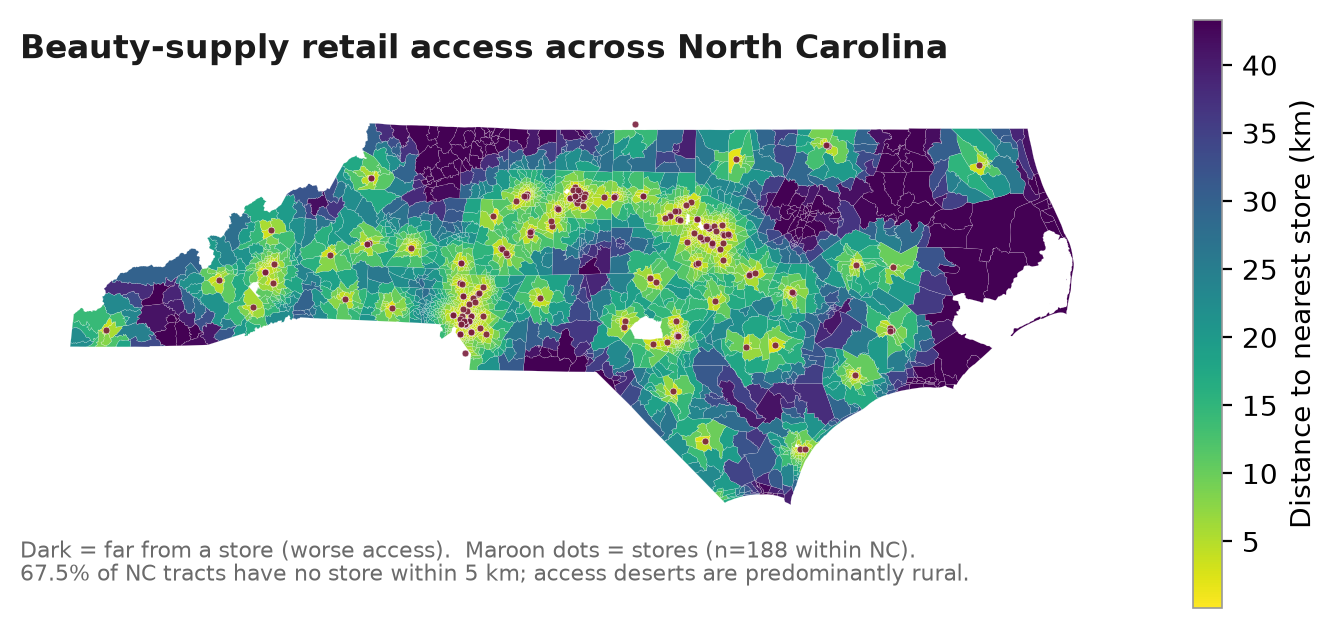
\includegraphics[width=\linewidth]{figures/fig1_nc_choropleth.png}
\caption{Distance from each census tract to the nearest beauty-supply store
across North Carolina (ACS 2022 tracts; stores from OpenStreetMap). Darker tracts
are farther from any store; maroon points are the 188 extracted stores inside the
state or within about 8~km of it. Access clusters in urban cores while rural counties form
contiguous access deserts.}
\label{fig:choropleth}
\end{figure}

\subsection{Spatial clustering}

Access was strongly and significantly clustered in space. Moran's~$I$ was
\textbf{0.92} for nearest-store distance and \textbf{0.83} for 5~km store count
(both pseudo-$p = 0.001$, 999 permutations), versus $0.66$ for percent-Black.
Retail access is thus even more spatially concentrated than the demographic
pattern itself.

\subsection{Access by neighborhood racial composition}

Contrary to a simple under-service hypothesis, access \emph{improved} as tract
percent-Black increased (Table~\ref{tab:quartile}). Tracts in the highest
percent-Black quartile were less than half as far from a store as those in the
lowest quartile and were far more likely to have a store within 5~km.

\begin{table}[H]
\centering
\caption{Beauty-supply access by quartile of tract percent-Black, North Carolina
(2{,}649 tracts). Higher percent-Black tracts have closer and more numerous
stores.}
\label{tab:quartile}
\small
\setlength{\tabcolsep}{5pt}
\resizebox{\textwidth}{!}{%
\begin{tabular}{lcccc}
\toprule
\textbf{Percent-Black quartile} & \textbf{Tracts} & \textbf{Median nearest store (km)} & \textbf{Mean stores within 5 km} & \textbf{\% tracts with no store in 5 km} \\
\midrule
Q1 (lowest \% Black)  & 663 & 14.2 & 0.68 & 81.7 \\
Q2                    & 662 & 9.2  & 0.97 & 70.1 \\
Q3                    & 662 & 8.7  & 0.98 & 64.0 \\
Q4 (highest \% Black) & 662 & 5.5  & 1.23 & 53.9 \\
\bottomrule
\end{tabular}}
\end{table}

\begin{figure}[H]
\centering
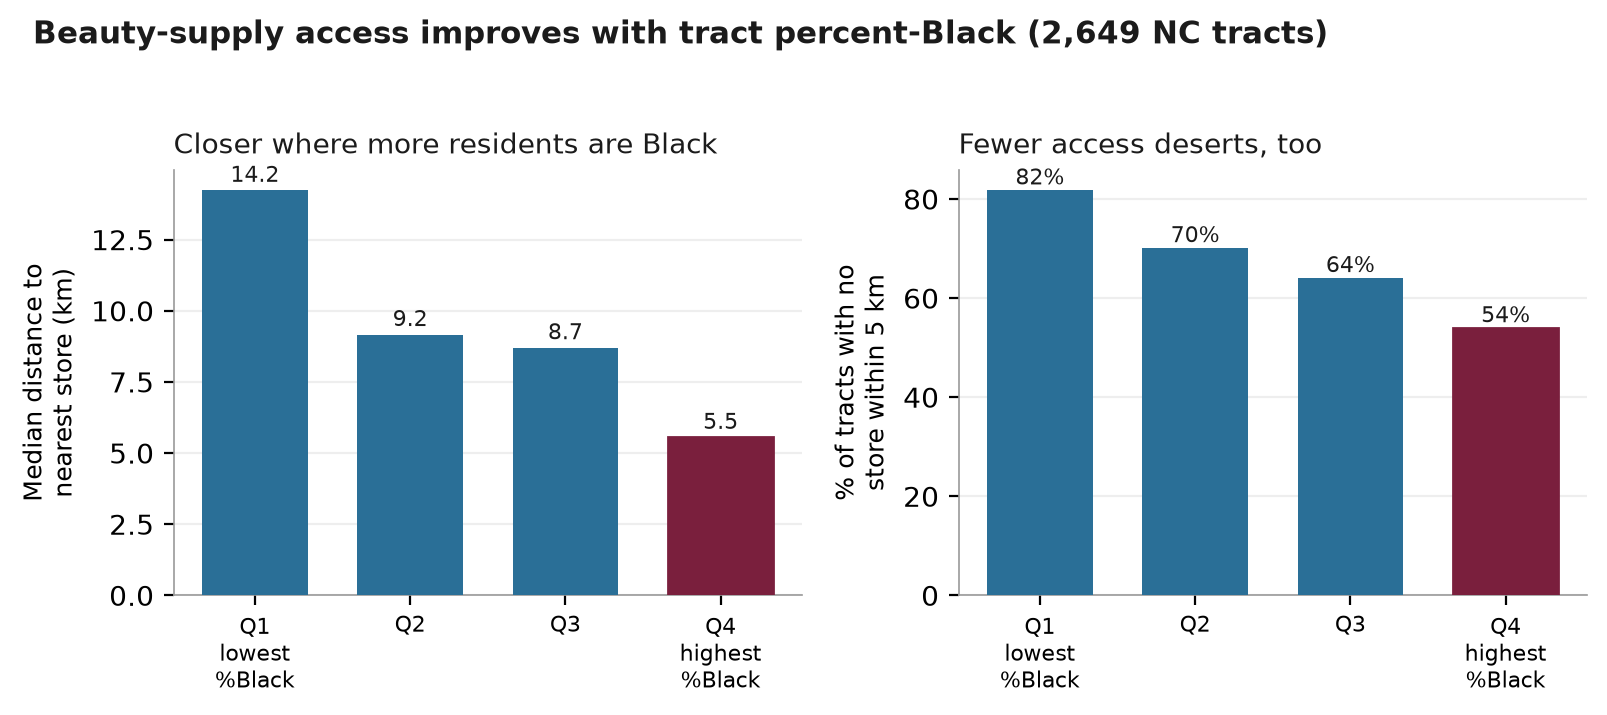
\includegraphics[width=\linewidth]{figures/fig2_quartile_gradient.png}
\caption{Beauty-supply access by quartile of tract percent-Black. Both
distance to the nearest store (left) and the share of tracts with no store
within 5~km (right) decrease monotonically as percent-Black rises; the
highest-percent-Black quartile (maroon) has the best access.}
\label{fig:quartile}
\end{figure}

Spearman correlations were consistent: percent-Black was negatively associated
with distance to the nearest store ($\rho = -0.21$) and positively with store
count ($\rho = 0.22$). In the negative-binomial model ($n = 2{,}624$ tracts with
complete covariates; dispersion fixed at 1), the expected 5~km store count rose
with percent-Black (incidence rate ratio [IRR] 1.02 per percentage point,
$p < 0.001$), poverty rate (IRR 1.02, $p < 0.001$), and median income (IRR 1.21
per \$10{,}000, $p < 0.001$). The associations kept their direction and
significance when dispersion was estimated by maximum likelihood (IRR 1.02 for
percent-Black, 1.02 for poverty, 1.24 for income) and when standard errors were
clustered by county (all $p < 0.001$). Access also tracked population density:
98.5\% of tracts in the lowest-density quartile had no store within 5~km (median
distance 22.6~km), compared with 24.2\% (3.1~km) in the highest-density quartile.
The percent-Black gradient therefore sits on top of a steep urban to rural gradient.

\subsection{Metropolitan case studies}

Five metropolitan areas were examined as county subsets of the statewide layer,
so that the same store set and ACS vintage apply throughout
(Table~\ref{tab:cities}, Figure~\ref{fig:metros}). Every metro had better access
than the state as a whole: the share of tracts with no store within 5~km ranged
from 22\% in Charlotte to 54\% in Fayetteville, against 67.5\% statewide. Access
remained significantly spatially clustered within every metro (Moran's~$I$ for
nearest-store distance 0.61 to 0.79, all pseudo-$p = 0.001$). Within-metro racial
gradients were modest and mixed. Majority-Black tracts were closer to the nearest
store than other tracts in Greensboro (median 2.4 vs 3.4~km), Raleigh (3.4 vs
3.8~km), and Fayetteville (4.4 vs 5.7~km), and slightly farther in Charlotte (3.5
vs 3.1~km) and Durham (4.3 vs 3.5~km). This pattern suggests that the strong
statewide gradient in Table~\ref{tab:quartile} reflects, at least in part, the
contrast between urban and rural counties rather than consistent sorting within
metros.

\begin{table}[H]
\centering
\caption{Metropolitan case studies (county subsets of the statewide layer, same
349-store extract and ACS 2022 vintage). ``\% no store'' is the share of tracts
with no store within 5~km. Moran's $I$ is for nearest-store distance
(pseudo-$p = 0.001$ in every row). Statewide shown for reference.}
\label{tab:cities}
\small
\setlength{\tabcolsep}{4pt}
\resizebox{\textwidth}{!}{%
\begin{tabular}{lcccccc}
\toprule
\textbf{Area} & \textbf{Tracts} & \textbf{Median \% Black} & \textbf{Median nearest (km)} & \textbf{\% no store in 5 km} & \textbf{Mean stores $\leq$5 km} & \textbf{Moran's $I$} \\
\midrule
North Carolina & 2{,}649 & 14.7 & 9.3 & 67.5 & 0.97 & 0.92 \\
Charlotte      & 302     & 29.8 & 3.2 & 22.2 & 3.11 & 0.79 \\
Raleigh        & 229     & 14.3 & 3.7 & 31.9 & 1.75 & 0.78 \\
Greensboro     & 125     & 29.4 & 3.0 & 29.6 & 4.18 & 0.70 \\
Durham         & 67      & 31.2 & 3.6 & 29.9 & 1.22 & 0.61 \\
Fayetteville   & 81      & 35.9 & 5.2 & 54.3 & 1.33 & 0.76 \\
\bottomrule
\end{tabular}}
\end{table}

\begin{figure}[H]
\centering
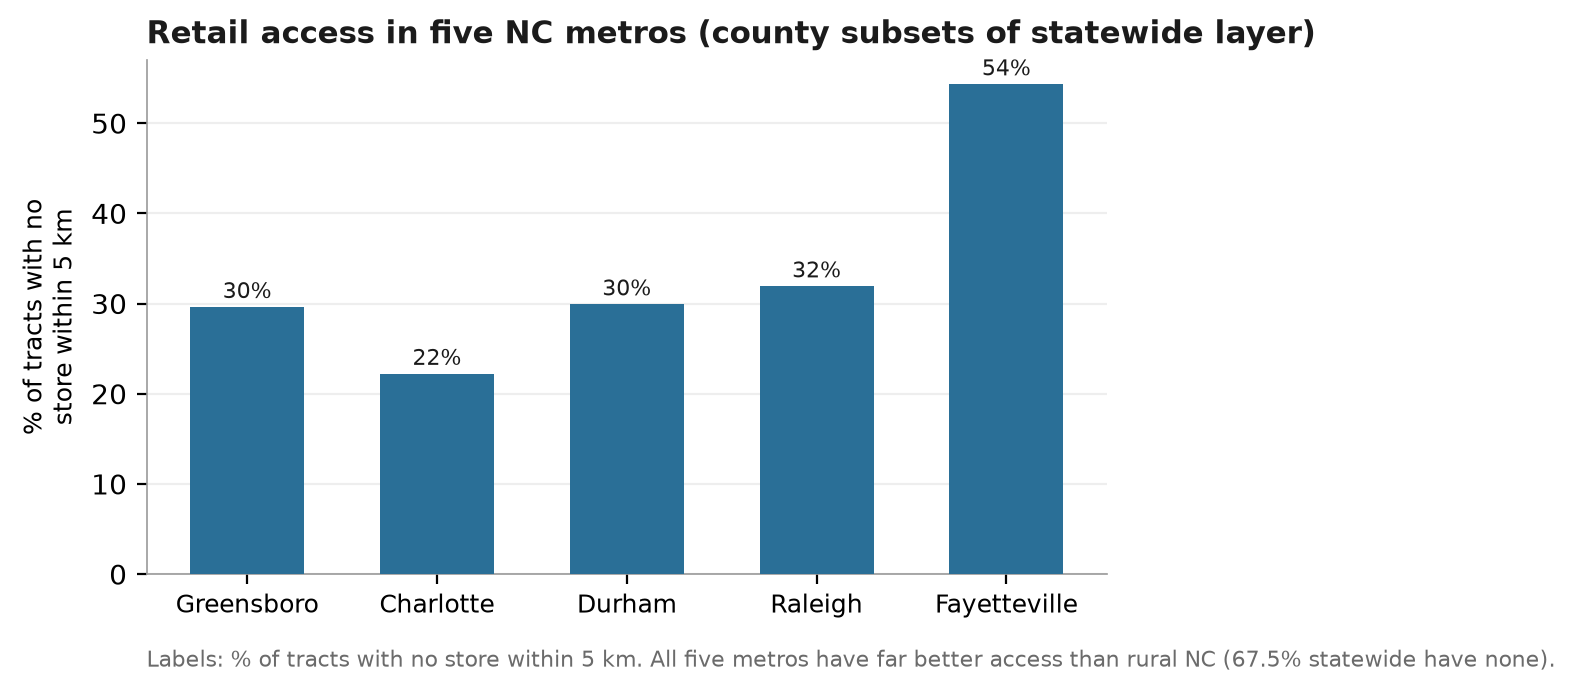
\includegraphics[width=0.92\linewidth]{figures/fig3_metros.png}
\caption{Share of tracts with no beauty-supply store within 5~km across five
North Carolina metros (county subsets of the statewide layer). Every metro has
better access than the state as a whole (dashed line, 67.5\%).}
\label{fig:metros}
\end{figure}

\section{Discussion}
\label{sec:discussion}

The clearest finding is that beauty-supply retail in North Carolina is highly
spatially concentrated and is \emph{more} available in Black and urban
neighborhoods, while two-thirds of the state's tracts, disproportionately
rural, lack a store within 5~km. This is consistent with beauty-supply stores
functioning as a targeted-market retail sector that locates where demand for
products such as hair adhesives is greatest. Framed as exposure opportunity,
the geography means the point-of-purchase for these prolonged-contact products
is most dense precisely in the communities already identified in the
biomonitoring literature as carrying elevated hair-product chemical burdens
\citep{helm2018,jamestodd2021,zota2017}. Greater availability is not the same as
greater risk, but it is where the opportunity for acquisition and repeated use
is concentrated, and therefore where exposure research and risk communication
would reach the most product-proximate populations.

This reframing matters because the naive environmental-justice expectation that
Black neighborhoods are \emph{under}-served does not hold for this retail class;
the data contradict it. Reporting the observed direction is itself part of the
contribution: access disparities here follow an urban to rural contrast layered
on a targeted-market concentration, not a simple race-based deficit.

\subsection{Limitations}

\begin{enumerate}
\item \textbf{Store data are incomplete and include out-of-state stores.}
Locations come from OpenStreetMap, a volunteer dataset that undercounts stores,
especially in rural areas and for independent retailers, and store counts varied
across extraction runs. The statewide extract appears to have been retrieved with
a bounding-box query: 161 of its 349 points lie more than about 8~km outside North
Carolina, and 156 of those fall inside the state's bounding box (for example
stores in Greenville and Spartanburg, South Carolina), leaving 183 stores inside
the state. Distances were computed against all 349 points, which lets tracts near
the state line use the nearest store across it, but the figure of 349 overstates
the number of North Carolina stores. Only stores inside or within about 8~km of
the state are drawn in Figure~\ref{fig:choropleth}. A validated business registry
(state licensing or a commercial listing such as Data Axle) is the clearest path
to defensible counts and is the top revision priority.
\item \textbf{Ecological design.} Tract-level access does not describe
individuals and is not purchase, use, dermal dose, or disease. No causal or
individual inference is warranted.
\item \textbf{Access is a crude proxy.} Distance from a tract centroid to the
nearest store, computed on planar coordinates in a single projected frame,
ignores road networks, travel mode, online purchasing, and within-tract
heterogeneity, and introduces mild geometric distortion over the full state
extent.
\item \textbf{Composite index is race-weighted by construction.} The underserved
index embeds percent-Black at a 0.40 weight and is used only for intervention
targeting, never as evidence of disparity; all disparity results rest on raw
access measures.
\item \textbf{Cross-sectional.} A single ACS vintage and a single store snapshot
cannot speak to change over time.
\item \textbf{No product verification.} Store categories were not field-verified
to stock hair adhesives specifically.
\end{enumerate}

\subsection{Implications and future work}

The maps provide a site-selection tool: the highest-access, higher-percent-Black
urban clusters are where recruitment for product sampling, biomonitoring, or
salon-worker studies would be most efficient, and where plain-language risk
communication would reach the most users. Priority extensions are (1) replacing
OpenStreetMap counts with a validated store registry; (2) network- rather than
straight-line distance; and (3) linking this access layer to the product-level
chemical and dermal-exposure analysis developed elsewhere in this project, so
that \emph{where} products are obtained can be joined to \emph{what} is in them.

\section{Conclusion}
\label{sec:conclusion}

Beauty-supply retail access in North Carolina is strongly spatially clustered and
concentrated in Black and urban neighborhoods, with large rural access gaps.
Interpreted as an exposure-opportunity proxy for hair-adhesive products, the
geography locates the communities most product-proximate to a class of
prolonged-contact cosmetics. This offers an evidence-based foundation for targeting
exposure research and risk communication, reported in the direction the data show
rather than the one assumed.

\section*{Data and code availability}
All code, input tables, and tract-level outputs are available in the project
repository. The folder \texttt{paper\_reproduction/} regenerates every statistic,
table, and figure in this paper from those files (\texttt{python reproduce.py}), and
\texttt{verify\_against\_paper.py} checks the numbers printed here against the
computed results.

\section*{Acknowledgments}
We thank [CONFIRM colleagues] for feedback. Store data \copyright{}
OpenStreetMap contributors (ODbL); demographic data from the U.S. Census Bureau
American Community Survey.

\bibliographystyle{plainnat}
\begin{thebibliography}{99}

\bibitem[Anselin(1995)]{anselin1995} Anselin, L. (1995). Local indicators of
spatial association: LISA. \textit{Geographical Analysis}, 27(2), 93-115.

\bibitem[Boatman et~al.(2026)]{boatman2026} Boatman, A.~K., Ferland, T.~M., \&
Whitehead, H.~D. (2026). \textit{Curated chemicals reported in consumer products
using non-targeted analyses (NTA)} [Data set]. UL Research Institutes, Chemical
Insights.

\bibitem[Dodson et~al.(2012)]{dodson2012} Dodson, R.~E., et~al. (2012). Endocrine
disruptors and asthma-associated chemicals in consumer products.
\textit{Environmental Health Perspectives}, 120(7), 935-943.

\bibitem[Helm et~al.(2018)]{helm2018} Helm, J.~S., et~al. (2018). Measurement of
endocrine disrupting and asthma-associated chemicals in hair products used by
Black women. \textit{Environmental Research}, 165, 448-458.

\bibitem[James-Todd et~al.(2021)]{jamestodd2021} James-Todd, T., et~al. (2021).
Racial/ethnic disparities in environmental endocrine disrupting chemicals and
women's reproductive health. \textit{Current Epidemiology Reports}.

\bibitem[Moran(1950)]{moran1950} Moran, P.~A.~P. (1950). Notes on continuous
stochastic phenomena. \textit{Biometrika}, 37(1/2), 17-23.

\bibitem[Walker et~al.(2010)]{walker2010} Walker, R.~E., Keane, C.~R., \&
Burke, J.~G. (2010). Disparities and access to healthy food in the United States:
A review of food deserts literature. \textit{Health \& Place}, 16(5), 876-884.

\bibitem[Zota \& Shamasunder(2017)]{zota2017} Zota, A.~R., \& Shamasunder, B.
(2017). The environmental injustice of beauty: Framing chemical exposures from
beauty products as a health disparities concern. \textit{American Journal of
Obstetrics and Gynecology}, 217(4), 418.e1-418.e6.

\end{thebibliography}

\end{document}
